\usetikzlibrary{bayesnet}
\scalebox{0.6}{
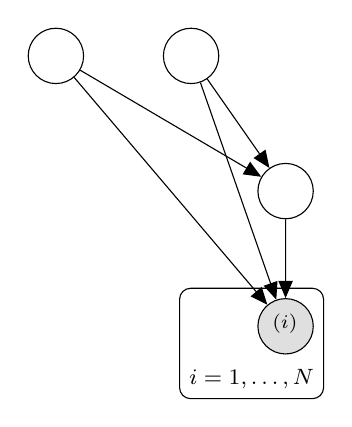
\begin{tikzpicture}[scale=3]

  % Define nodes
  \node[latent] (W) {$\mW$};
  \node[latent, left=of W] (p) {$\vp$};
  \node[latent, below=of W, xshift=1.2cm] (Theta) {$\mTheta$};
  \node[obs, below=of Theta] (x) {$\vx^{(i)}$};
  
  % Connect nodes
  \edge {p} {x};
  % \edge {p} {W};
  \edge {W} {Theta};
  \edge {W} {x};
  \edge {Theta} {x};
  \edge {p} {Theta};
  
  % Define plate
  \plate {x_plate} {(x)} {$i = 1, \dots, N$};

\end{tikzpicture}
}